\documentclass{homework}
\usepackage[utf8]{inputenc}
\usepackage{amsmath}
\usepackage{amssymb}
\usepackage{braket}
\usepackage{hyperref}
\hypersetup{
    colorlinks=true,
    linkcolor=blue,
    filecolor=magenta,      
    urlcolor=cyan,
    pdftitle={Overleaf Example},
    pdfpagemode=FullScreen,
    }

% package for source code highlighting
\usepackage{minted}


% CHANGE THE FOLLOW THREE LINES!
\newcommand{\hwname}{Marek Böhm}
\newcommand{\hwemail}{marek.bhm@seznam.cz}
\newcommand{\hwnum}{}

% CHANGE THESE ONLY ONCE PER CLASS
\newcommand{\hwtype}{Workshop předmětu Návrhové vzory 19.6. - 20.6. 2021}
\newcommand{\hwclass}{}

\begin{document}

\maketitle

\question*{Marek Böhm - Adaptér }

Dochází k validaci kódu vstupenky vzhledem ke kódu vstupenky uloženým v databázi a k uložení události do databáze. Pokud je validace úspěšná, dojde k zaslání kladného výsledku validace a k otevření turniketu. 

\question*{High level návrh systému}

\begin{center}
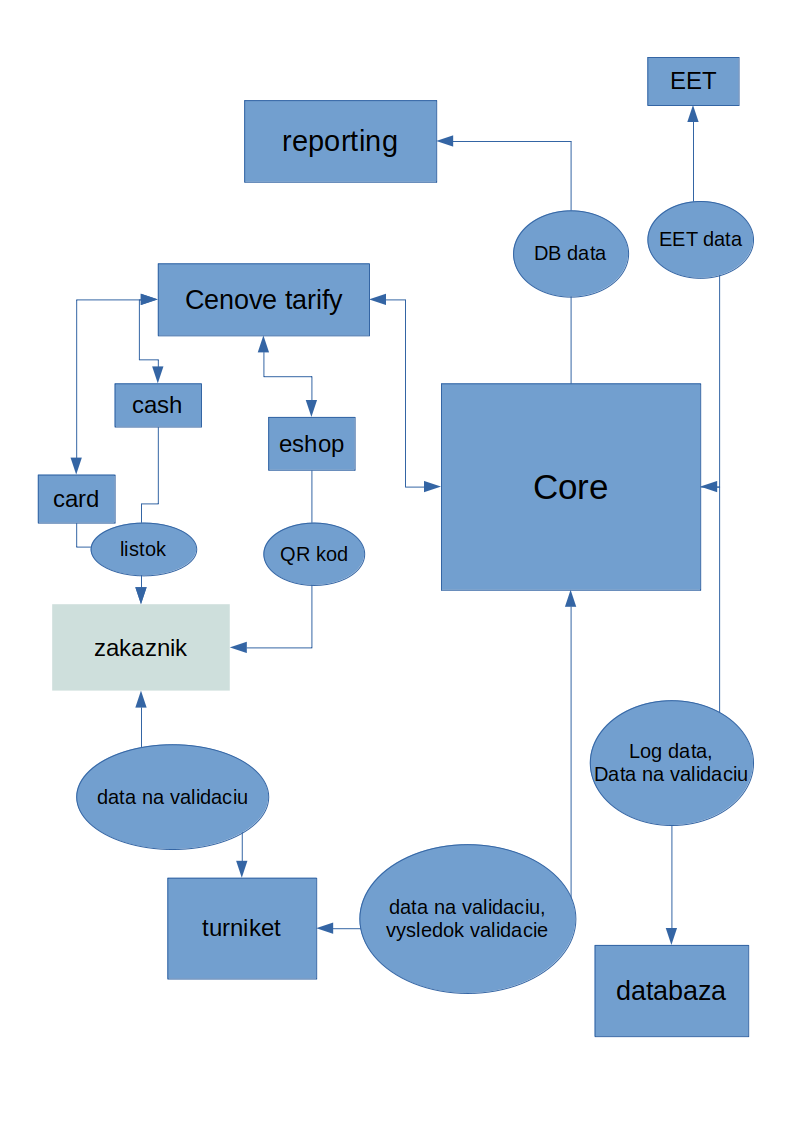
\includegraphics[scale=0.25]{high_level_nakres.png}
\end{center}

\question*{Teorie a definice vzoru adaptér}

Vzor adaptér lze definovat následujícím způsobem:

Vzor adaptér převádí rozhraní třídy na jiné rozhraní, které klienti očekávají. Adaptér umožňuje třídám spolupracovat, což by jinak kvůli nekompatibilním rozhraním nemohly.

Adaptéry se používají, když máme třídu (\textbf{Klient}), která očekává nějaký typ objektu, a máme objekt (\textbf{Adaptér}), který nabízí stejné funkce, ale vystavuje jiné rozhraní.Při použití Adaptéru Klientem dojde k proběhnutí následujících kroků:

\begin{enumerate}
  \item Klient provede požadavek na adaptér voláním metody adaptéru pomocí cílového rozhraní.
  \item Adaptér přeloží tento požadavek pro osvojence (\textbf{Adaptee}) pomocí rozhraní osvojence (Adaptee)
  \item Klient obdrží výsledky volání metody a neví o existenci Adaptéru
\end{enumerate}

Obecný diagram vzoru Adaptér vypadá následujícím způsobem:

\begin{center}
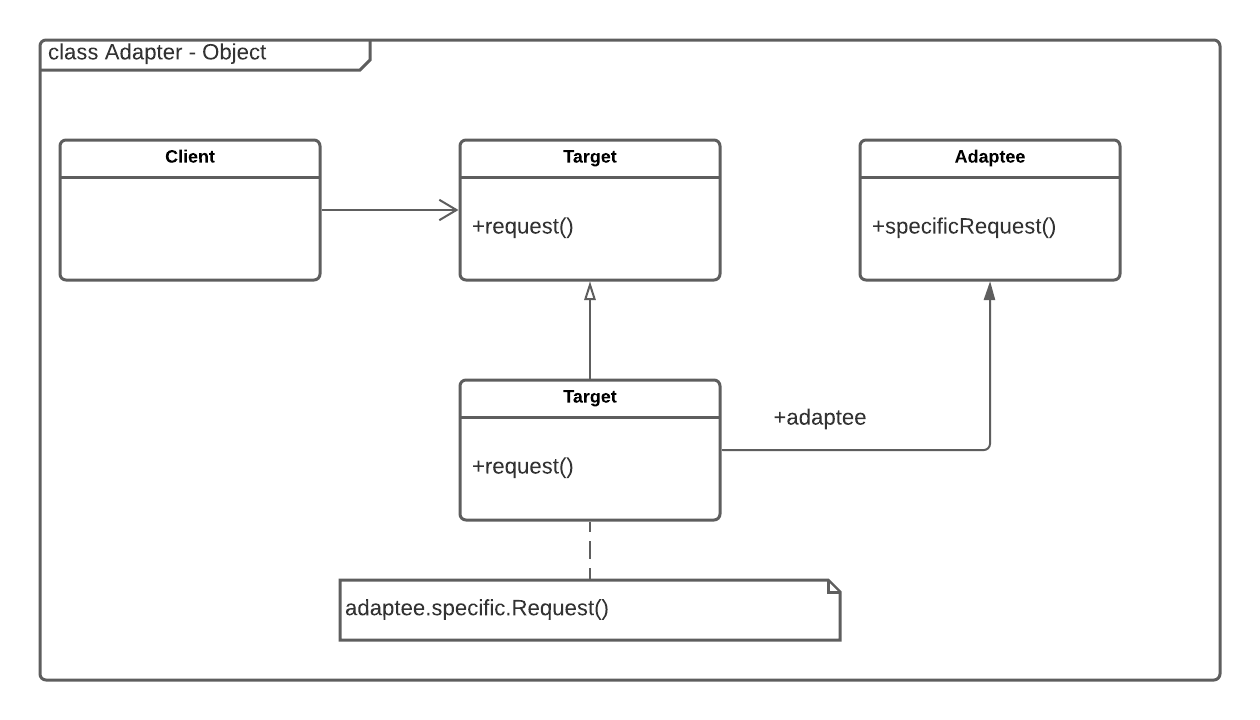
\includegraphics[scale=0.75]{Adapter.png}
\end{center}

Více informací o návrhovém vzoru adaptér lze nalézt zde:

\href{https://uuapp.plus4u.net/uu-bookkit-maing01/f0b1d8809f3a436fb5413d9ea3226277/book/page?code=38722233}{uuBook Design Patterns}

\question*{Vysvětlení použití návrhového vzoru:}

\begin{itemize}

  \item Na co byl návrhový vzor použit a proč byl zvolen
  \item Posouzení vhodnosti a výhody
  \item Možné alternativy použití
  
  \begin{itemize}
  
  \item Bridge
  \item Decorator
  \item Proxy
  
  \end{itemize}
  
\end{itemize}

\question*{Pseudo kód - Java-like syntaxe}

\begin{minted}{java}

// Java implementation of Adapter pattern

interface Bird
{
	// birds implement Bird interface that allows
	// them to fly and make sounds adaptee interface
	public void fly();
	public void makeSound();
}

class Sparrow implements Bird
{
	// a concrete implementation of bird
	public void fly()
	{
		System.out.println("Flying");
	}
	public void makeSound()
	{
		System.out.println("Chirp Chirp");
	}
}

interface ToyDuck
{
	// target interface
	// toyducks dont fly they just make
	// squeaking sound
	public void squeak();
}

class PlasticToyDuck implements ToyDuck
{
	public void squeak()
	{
		System.out.println("Squeak");
	}
}

class BirdAdapter implements ToyDuck
{
	// You need to implement the interface your
	// client expects to use.
	Bird bird;
	public BirdAdapter(Bird bird)
	{
		// we need reference to the object we
		// are adapting
		this.bird = bird;
	}

	public void squeak()
	{
		// translate the methods appropriately
		bird.makeSound();
	}
}

class Main
{
	public static void main(String args[])
	{
		Sparrow sparrow = new Sparrow();
		ToyDuck toyDuck = new PlasticToyDuck();

		// Wrap a bird in a birdAdapter so that it
		// behaves like toy duck
		ToyDuck birdAdapter = new BirdAdapter(sparrow);

		System.out.println("Sparrow...");
		sparrow.fly();
		sparrow.makeSound();

		System.out.println("ToyDuck...");
		toyDuck.squeak();

		// toy duck behaving like a bird
		System.out.println("BirdAdapter...");
		birdAdapter.squeak();
	}
}

\end{minted}{java}

\end{document}
